\documentclass[12pt,letterpaper]{scrartcl}
\usepackage{lipsum}
\usepackage[utf8]{inputenc}
\usepackage{amsmath}
\usepackage{amsfonts}
\usepackage{amssymb}
\usepackage{graphicx}
\usepackage[left=3cm,right=2.5cm,top=2.5cm,bottom=2.5cm]{geometry}
\usepackage[]{algorithm2e}
\author{Don cuyi}

%Color
\usepackage{color}
\definecolor{nred}{RGB}{174,49,54}
\definecolor{nblue}{RGB}{86,99,146}
\definecolor{nalgo}{RGB}{188,139,76}
\usepackage{sectsty}
\sectionfont{\color{nred}}
\subsectionfont{\color{nblue}}
\subsubsectionfont{\color{nalgo}}

%Librías tikz
\usepackage{pgf,tikz}
\usepackage{mathrsfs}
\usetikzlibrary{arrows}
\usetikzlibrary[patterns]
\newcommand{\degre}{\ensuremath{^\circ}}
\definecolor{qqwuqq}{rgb}{0.,0.39215686274509803,0.}
\definecolor{ffttww}{rgb}{1.,0.2,0.4}
%Hipervinculos
\usepackage{hyperref}

\usepackage{fancyhdr}
\pagestyle{fancy}
\fancyhead[L]{Combinatoria}
\fancyhead[C]{Licenciatura en ciencias de la computación}
\fancyhead[R]{USACH}

%interlineado
\renewcommand{\baselinestretch}{1.2}

%\bibitem{Yahoo} \textsc{Andres G} (2009),
%\textbf{¿Generar números aleatorios negativos en Lenguaje C?} En \textsc{Yahoo! respuestas}
%Recuperado el el 23 del julio del 2014
%\url{https://es.answers.yahoo.com/question/index?qid=20091121055249AAUQH3N}

\newcommand{\biblio}[7]{
\bibitem{#1} \textsc{#2} (#3),
\textbf{#4} En \textsc{#5}
Recuperado el #6
\url{#7}
}

% Last, F. M. (Year Published) Book. City, State: Publisher.
\newcommand{\book}[5]{
\bibitem{#1} \textsc{#2} (#3),
\textbf{#4}  \textsc{#5} Estado: Publicado
}

\begin{document}

\begin{titlepage}

	\begin{center}

		{\Large { Licenciatura en ciencia de la computación} }

		
\includegraphics[scale=1]{UDSCNRJ}
		\\[1cm]

		{\Huge \textsc{Algoritmo Euclideano}}\\[0.7cm]

		{\huge  Matemática Computacional}\\[2cm]


		\begin{minipage}[l]{0.4\textwidth}
			\begin{flushleft}
				\linespread{1}
				\textbf{\textsf{Profesor:}}\\
				\large Nicolas Thériault
			\end{flushleft}
		\end{minipage}
		\begin{minipage}[l]{0.4\textwidth}

			\begin{flushright}

				\textbf{\textsf{Autor:}}\\
				\linespread{1}
				\large Sergio Salinas\\
				\large Danilo Abellá\\

			\end{flushright}
		\end{minipage}

	\end{center}

\end{titlepage}



\newpage
\section*{Introducción}


\section{Tiempos de ejecución de Algoritmo}

A continuación se mostrarán los tiempos de ejecución apra cada valor de "n" y "p" respectivamente.

\subsection{Tiempos de ejecución para valores de "n" y "p".}

Costos computacionales de los algoritmos donde: \[p \in \{1/10, 3/10, 1/2, 7/10, 9/10\} \] para distintos valores de n:
\\\\
n=18
\\\\
p=0.1\hspace{1cm}57.0000000
\\
p=0.3\hspace{1cm}43.0000000
\\
p=0.5\hspace{1cm}41.0000000
\\
p=0.7\hspace{1cm}128.0000000
\\
p=0.9\hspace{1cm}40.0000000
\\\\
n=660
\\\\
p=0.1\hspace{1cm}18815.0000000
\\
p=0.3\hspace{1cm}18698.0000000
\\
p=0.5\hspace{1cm}26974.0000000
\\
p=0.7\hspace{1cm}18506.0000000
\\
p=0.9\hspace{1cm}21156.0000000
\\\\
n=8000
\\\\
p=0.1\hspace{1cm}2890310.0000000
\\
p=0.3\hspace{1cm}3851808.0000000
\\
p=0.5\hspace{1cm}5042122.0000000
\\
p=0.7\hspace{1cm}6085456.0000000
\\
p=0.9\hspace{1cm}6920520.0000000
\\\\
\subsection{Costo computacional para n = 1000.}

Costos computacionales de los algoritmos para n = 1000 para distintos valores de p.
\\
Tiempos de espera para los siguientes valores de "p":
\\\\
p=0\hspace{1cm}34094.0000000
\\
p=0.1\hspace{1cm}31610.0000000
\\
p=0.2\hspace{1cm}37190.0000000
\\
p=0.3\hspace{1cm}55043.0000000
\\
p=0.4\hspace{1cm}47476.0000000
\\
p=0.5\hspace{1cm}45258.0000000
\\
p=0.6\hspace{1cm}46934.0000000
\\
p=0.7\hspace{1cm}56155.0000000
\\
p=0.8\hspace{1cm}56874.0000000
\\
p=0.9\hspace{1cm}47229.0000000
\\
p=1\hspace{1cm}48239.0000000


\newpage
\section{Formulación experimentos}

\section{Repretesentación de grafo utilizada}

Se utilizo una matriz de adyacencia para representar el grafo debido a que en C se puede manejar sencillamente como un arreglo de dos dimensiones. De esta forma escribir y recorrer la matriz fue tan sencillo como recorrer una matriz de largo n, donde n es la cantidad de vértices que coincide con la cantidad de filas y columnas de va a tener la matriz.

\section{Algoritmo de busqueda de camino}

La principal razón porque la la búsqueda de ciclo de euler da un ciclo un de euler es debido a que en el grafo generado todas los vértices tienen grado par.

Para crear el algoritmo se utilizo una función recursiva para recorrer el grafo y borrar las aristas entre los vértice y una estrategia de backtracking para volver un paso atrás en el caso de que haya llegado a un vértice sin aristas y aun hayan vértice que no se han recorrido. El algoritmo hace lo siguiente.

Al inicio de la función recursiva se posiciona en la fila y columna 0, a partir de ahí comienza a recorrer la fila hasta encontrar un 1, eso significa que hay una arista entre el vértice que esta representando la fila y el vértice que representa la columna, por lo cambia el 1 por un 0, al ser una matriz simétrica se borra en la posición transpuesta también. Después se va a la intercambia la posición de la fila por la columna y se empieza a recorrer esa fila desde la posición 0. el algoritmo continua así hasta que se recorre toda la matriz solo tenga 0 o hasta que se llegue a una fila llena de unos.

En el caso de que llegue a una fila llena de ceros significa que o que se encontró el camino euleriano o que se borraron todas las aristas de ese vértice y aun faltan aristas por recorrer en los otros vértices.

En el primer caso se termina el algoritmo y se muestra el camino. En el segundo se debe hacer un backtracking, para ello se ve el arreglo en el que se guardaba el camino euleriano y se vuelven a poner 1 donde se habían por 0, luego se va a última fila que se recorrió, pero en vez se partir desde la posición 0, esta vez se parte desde la posición siguiente al 0 que se borro, de esta forma se puede seguir recorriendo el grafo sin problemas hasta que ya se haya recorrido todas las aristas.






\section{Información de Hardware y Software}

\subsection{ Notebook - Danilo Abellá}
\subsubsection{Software}
\begin{itemize}
	\item SO: Xubuntu 16.04.1 LTS
	\item GMP Library
	\item Mousepad 0.4.0
\end{itemize}

\subsubsection{Hardware}
\begin{itemize}
	\item AMD Turion(tm) X2 Dual-Core Mobile RM-72 2.10GHz
	\item Memoria (RAM): 4,00 GB(3,75 GB utilizable)
	\item Adaptador de pantalla: ATI Raedon HD 3200 Graphics
\end{itemize}



\subsection{Notebook - Sergio Salinas}
\subsubsection{Software}
\begin{itemize}
	\item  SO: ubuntu Gnome 16.04 LTS
	\item Compilador: gcc version 5.4.0 20160609
	\item Editor de text: Atom
\end{itemize}

\subsubsection{Hardware}
\begin{itemize}
	\item Procesador: Intel Core i7-6500U CPU  2.50GHz x 4
	\item Video: Intel HD Graphics 520 (Skylake GT2)
\end{itemize}


\newpage

\section{Curvas de desempeño de resultados}
\subsection{Comportamiento para los valores de "p" pedidos.}

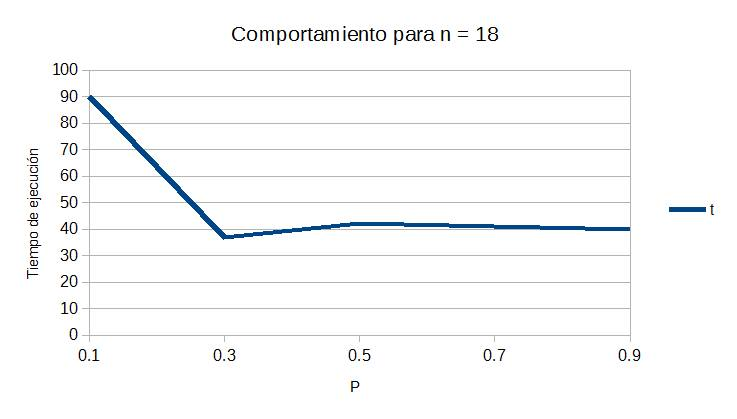
\includegraphics[scale=0.55]{n}

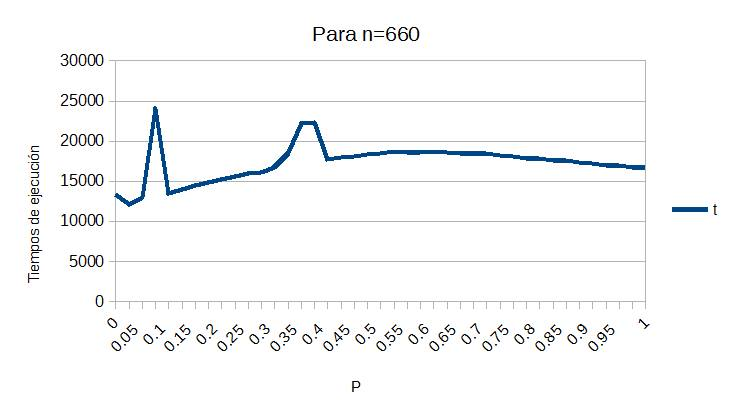
\includegraphics[scale=0.55]{nn}

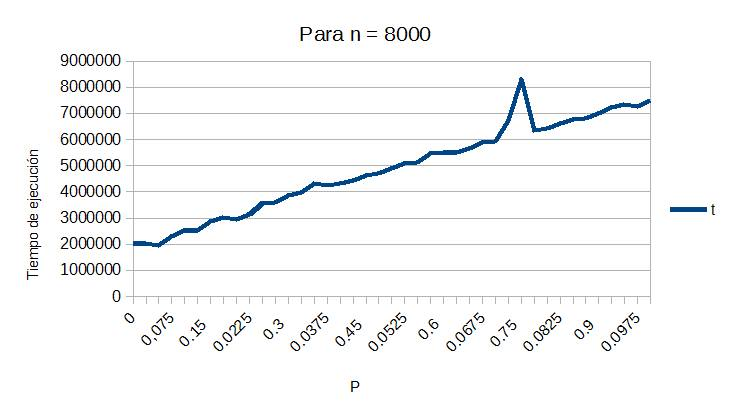
\includegraphics[scale=0.55]{nnnn}

\subsection{Costos computacionales de los algoritmos para n = 1000 para distintos valores de "p".}

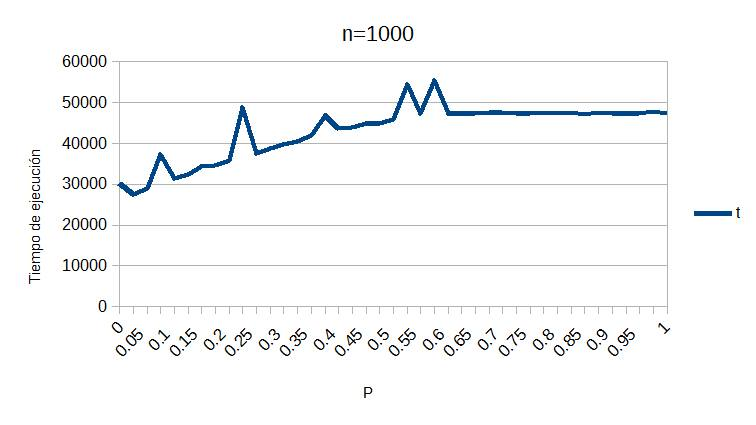
\includegraphics[scale=0.55]{nnn}

\newpage
\section{Conclusiones}

Con los datos recopilados de los gráficos podemos concluir que mientras mayor sea el valor de "n" mayor tiempo de ejecución se requiuere.
\\\\
También cave decir que independiente de "n" mientras mayor sea el valor de "p" el tiempo de ejecución también tiende siempre a aumentar , lo que quiere decir que ambas variables influyen en el tiempo de ejecución.
\\\\
Otro punto a considerar es que cuando "n" no es tan grande (apróx. menor a 1000) la variable "p" no es tan influyente , sin embargo cuando "n" toma un valor grande (apróx. mayor a 1000) "p" tiene mucha mas influencia en el tiempo de ejecución.

\end{document}
